%Micah Chambers

\documentclass{beamer}

\mode<presentation>
{
  \usetheme{Darmstadt}
  % or ...

  \setbeamercovered{transparent}
  % or whatever (possibly just delete it)
}
\usefonttheme[onlylarge]{structurebold}
\setbeamerfont*{frametitle}{size=\normalsize,series=\bfseries}
\setbeamertemplate{navigation symbols}{}
\setbeamercovered{transparent}


\usepackage[english]{babel}
% or whatever

\usepackage[latin1]{inputenc}
% or whatever

\usepackage{graphics}
\usepackage{times}
\usepackage[T1]{fontenc}
\usepackage[small]{caption}

\title{A Crash Course in FMRI Imaging}

\subtitle{Or More than you ever wanted to know about FMRI}

\author{Micah Chambers}

\institute {
  Bradley Department of Electrical and Computer Engineering\\
  Virginia Tech University}

\subject{Medical Imaging}

% If you have a file called "university-logo-filename.xxx", where xxx
% is a graphic format that can be processed by latex or pdflatex,
% resp., then you can add a logo as follows:

\pgfdeclareimage[height=0.5cm]{university-logo}{VT_marn_she_invent_cmyk}
\logo{\pgfuseimage{university-logo}}


% If you wish to uncover everything in a step-wise fashion, uncomment
% the following command: 

%\beamerdefaultoverlayspecification{<+->}


\begin{document}
\begin{frame}
  \titlepage
\end{frame}

\begin{frame}{Outline}
  \tableofcontents
  % You might wish to add the option [pausesections]
\end{frame}

\section{About FMRI}
\subsection{FMRI Basics}
\begin{frame}{Pulse Sequence}
  % - A title should summarize the slide in an understandable fashion
  %   for anyone how does not follow everything on the slide itself.
  
  \begin{itemize}
    \item $T2*$ Weighted Image, acquired either line by line or 
         with spiral sequence.
    \item One or more more slices are captured in a single reptition time (TR).
    \item Echo Planar Pulse Sequence, slices acquired in less than a
        tenth of a second, depending on resolution, etc.
    \item A full volume can usually be acquired in 2 to 4 seconds.
  \end{itemize}
  \begin{figure}
  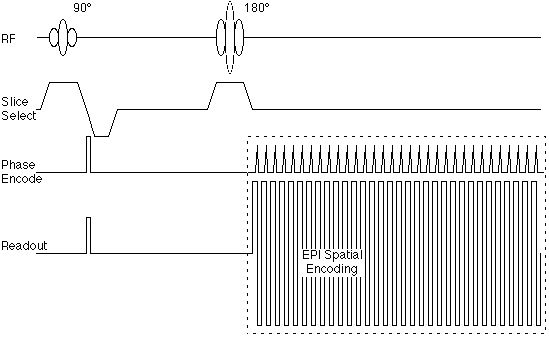
\includegraphics[scale=.23]{epi}
  \caption{
    \tiny
    \href{http://airto.hosted.ats.ucla.edu/BMCweb/BMC_BIOS/MarkCohen/Papers/EPI-fMRI.html}
    {http://airto.hosted.ats.ucla.edu/} }
  \end{figure}
\end{frame}

\subsection{The Bold Response}
\begin{frame}{Visualization of the BOLD Response}
\begin{figure}
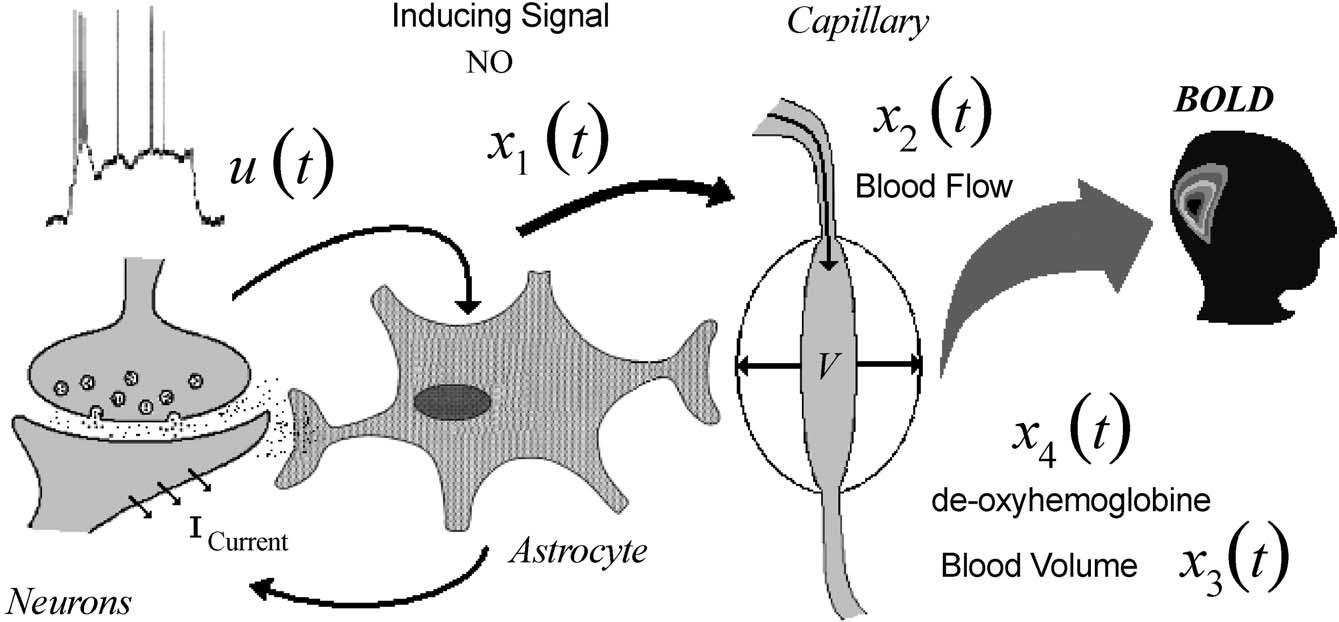
\includegraphics[scale=.23]{model}
\caption{
    \tiny
    \cite{ISI:000189252300007}
}
\end{figure}
\end{frame}

\begin{frame}{Equations}
  \begin{itemize}
    \item Normalized Cerebral Blood Flow:
    $$\ddot{f}(t) = \epsilon u(t) - \dot{f}(t)/\tau_s - (f(t)/\tau_f - 1)$$
    \item Normalized Cerebral Blood Volume:
    $$\dot{v}(t) = (1/\tau_0)( f(t) - v(t) ^ {1/\alpha}) $$
    \item Normalized Deoxyhaemoglobin Content:
    $$\dot{q}(t) = \frac{1}{\tau_0}\left(\frac{f(t)(1- (1-E_0)^{1/f(t)})}{E_0} - 
            \frac{q(t)}{v(t)^{1-1/\alpha}}\right)$$
    \item Hemodynamic Response - BOLD Signal
    $$y(t) = V_0(a_1( 1 - Q(t)) - a_2(1 - V(t)))$$
  \end{itemize}
\end{frame}


\subsection{Practical Concerns}
\begin{frame}{Pros and Cons}
  \begin{itemize}
    \item Benefits
    \begin{itemize}
        \item In Comparison to EEG/MEG very good resolution.
        \item Unlike MEG or EEG Image reconstruction is a known/solved problem.
    \end{itemize}
    \item Drawbacks
    \begin{itemize}
      \item Measures the result of a long chain of activations
      \begin{itemize}
        \item Exact variables and parameters are unknown and are
            difficult to calculate.
        \item Significant Amount of Lag between activation
            and a measurable output - can be as much as 8 seconds.
      \end{itemize}
      \item Slow Temporal Resolution
      \item Extremely Low Signal-to-Noise Ratio 
    \end{itemize}
  \end{itemize}
\end{frame}

\begin{frame}{Drawbacks Continued}
   \begin{itemize}
      \item Non-Gaussian, non-stationary Noise, Caused by:
      \begin{itemize}
        \item Physiological Interference
        \item Interference from the scanner
        \item Other, as yet unknown, factors
        \item See \cite{ISI:000080539300008} and \cite{ISI:000246766700003}
      \end{itemize}
  \end{itemize}
\begin{figure}
    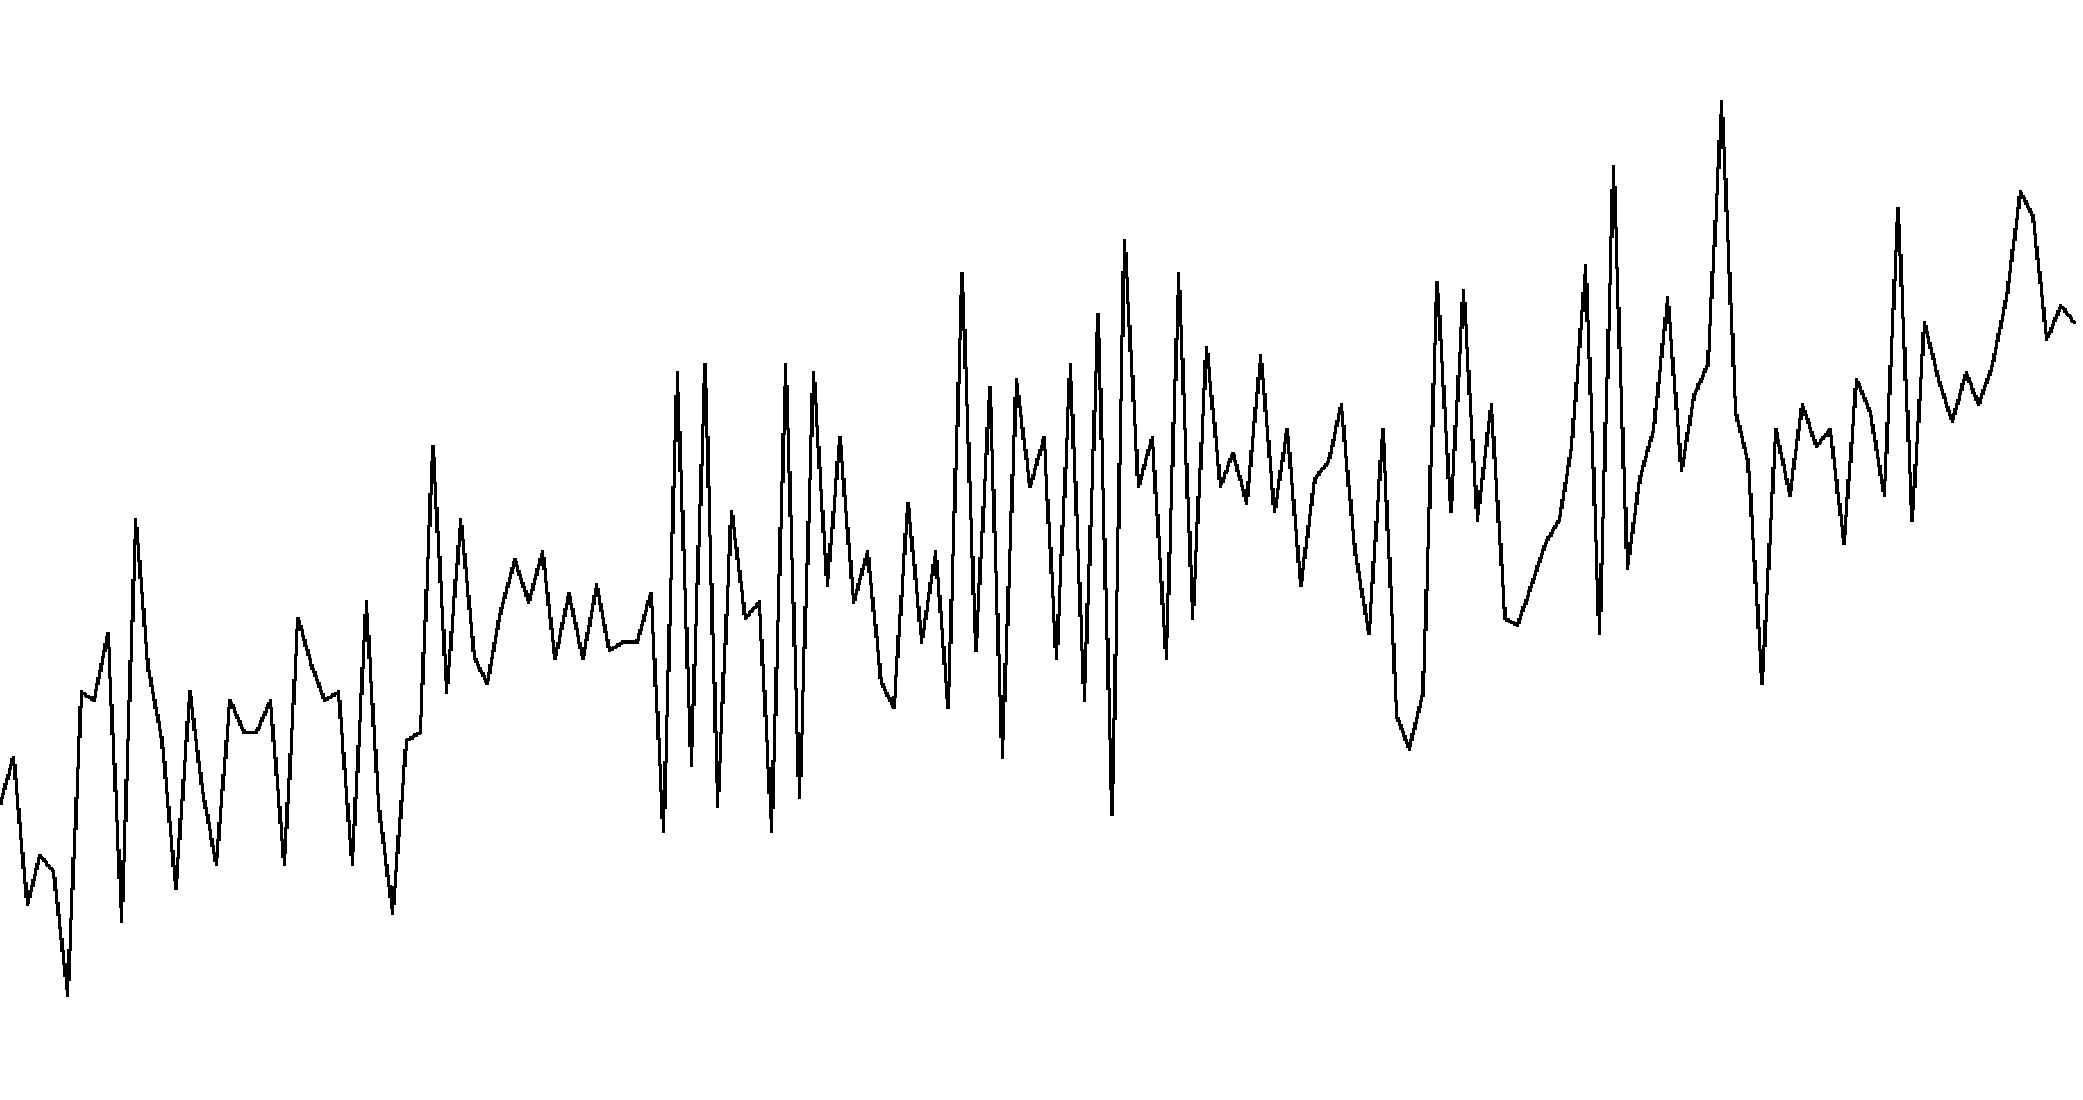
\includegraphics[scale=.15]{timeseries.png}
\end{figure}
\end{frame}
    
\section{Processing}
\subsection{Preprocessing}
\begin{frame}{Preprocessing}
\begin{itemize}
    \item Gaussian Filters especially when using the General Linear Model
    \item Removing Drift
    \begin{itemize}
        \item Extremely necessary, otherwise p value must be set prohibitively low. \cite{ISI:000246766700003}
        \item High Pass filters
        \item Various De-Trending methods 
        \begin{itemize}
            \item Polynomial fit
            \item Spline Fit
            \item Subtracting the Mean from the Timeseries
            \item Wavelets
        \end{itemize}
    \end{itemize}
     \item Detrended signals are often normalized using \%Difference.
    \item per-activation normalization
    \begin{itemize}
        \item Average signal for a few samples before activation \emph{should} begin.
    \end{itemize}
\end{itemize}
\end{frame}

\subsection{Linear Processing}
\begin{frame}{The General Linear Model}
\begin{itemize}
    \item Uses linear methods to extract useful information
    \item Can be effective for certain types of signal
    \item Used in many of the classical studies to determine regions
        associated with various tasks.
    \item Limited in dealing with complicated tasks.
    \item Utilizes Statistical Parameter Maps used to create clusters, then find 
        clusters not likely to have arisen randomly. (Random Field Theory)
    \item SPM is the standard tool for performing linear analysis.
\end{itemize}
\end{frame}

\subsection{Nonlinear Processing}
\begin{frame}{Nonlinear Analysis}
\begin{itemize}
    \item Use nonlinear state evolution models to determine activation.
    \item Removal of drift still necessary.
    \item Typically Rely on some sort of gradient decent technique to determine
        model parameters.
    \item Neural Networks
    \begin{itemize}
        \item Good at gathering disparate low SNR signals into meaningful information. 
        \item The method typically used by people studying visual cortex to "read" images from 
            a persons brain.
        \item Needs some method of removing irrelevant voxel data, to prevent over-fitting.
    \end{itemize}
    \item Particle Filters
    \begin{itemize}
        \item Based on real biological systems - recall the BOLD state equations
        \item Able to determine underlying state variables
        \item Tolerant of Noisy readings
    \end{itemize}
\end{itemize}
\end{frame}

\begin{frame}{BOLD Model}
\begin{itemize}
    \item The Balloon Model proposed by \cite{ISI:000073759600002} is the basic model.
    \item There are more complicated versions of the BOLD model:
    \begin{itemize}
        \item \cite{ISI:000240969200015} Reviews several existing models
        \item \cite{Buxton2004S220} Pioneered the Balloon model which was shown in the beginning.
        \item \cite{ISI:000234015300018} Adds interesting neural activation and a habituation model
        \item Some models loosen the link between CMRO2 (oxygen metabolism)
            and Cerebral Blood Flow - likely due to several papers that report
            such a decoupling.
    \end{itemize}
\end{itemize}
\end{frame}

\begin{frame}{Post Stimulus Undershoot Controversy}
\begin{itemize}
    \item The delinking of CMRO2 from CBF is postulated based on the "Post Stimulus Undershoot"
    \begin{itemize}
        \item In 2008 several papers claimed prove CBV and CBF both returned
            to normal before the BOLD signal, implying a decoupling of CBV from the BOLD signal.
        \item In November of 2008, \cite{ISI:000265938700001} went out of the way to refute such a de-coupling,
            claiming that other experiments were catching Arterial CBV rather than Venous CBV.
        \item In \cite{ISI:000240969200015} (2004), it was shown that merely adding volume viscosity to
            the BOLD equations was sufficient to account for much of the undershoot.
    \end{itemize}
\end{itemize}
\end{frame}

\begin{frame}{Model Comparisons}
\begin{figure}
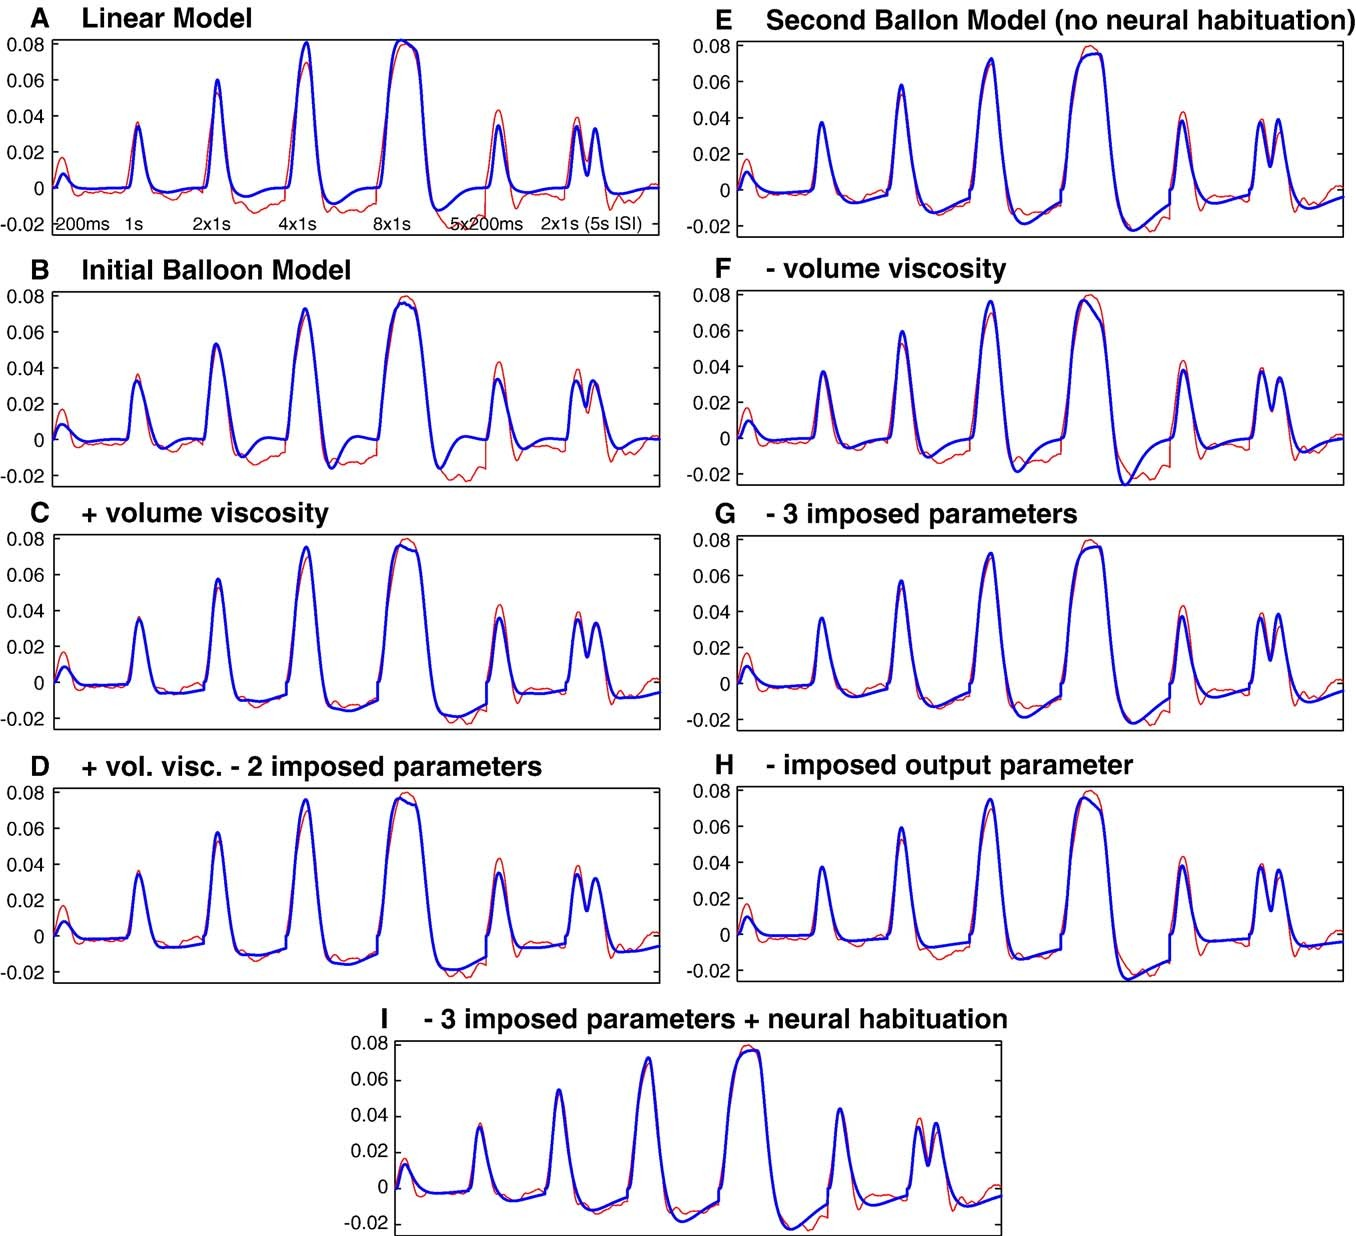
\includegraphics[scale=.165]{demeux}
\end{figure}
\end{frame}

\section{Conclusion}
\begin{frame}{The Future of FMRI}
\begin{itemize}
    \item Extremely Powerful tool.
    \item Better Models are increasing FMRI's flexibility.
    \item Combining FMRI with other methods of imaging will add 
        extensive knowledge to the understanding of how the human brain
        works.
    \item Much of the newer research is based around non-linear non-Gaussian
        models.
\end{itemize}
\end{frame}

% All of the following is optional and typically not needed. 
\appendix
\section{References}

% All of the following is optional and typically not needed. 
\appendix
\section<presentation>*{\appendixname}
\subsection<presentation>*{For Further Reading}

\begin{frame}[allowframebreaks]
  \bibliographystyle{abbrvnat}
  \bibliography{references}
\end{frame}

\end{document}


